%%%%%%%%%%%%%%%%%%%%%%%%%%%%%%%%%%%%%%%%%%%%%%%%%%%%%%%%%%%%%%%%%%%%%%%%%%%%%%%%
%                                                                              %
%   PAW   - Reference Manual -- LaTeX Source                                   %
%                                                                              %
%   Chapter 7: HBOOK                                                           %
%                                                                              %
%   EPS file : pawstor.eps                                                     %
%              hbzebra.eps                                                     %
%              hbbatch.eps                                                     %
%              fhtest1.eps                                                     %
%              fgcuts.eps                                                      %
%              fhtest2.eps                                                     %
%              fhtest3.eps                                                     %
%              fhtest4.eps                                                     %
%              fhtest5.eps                                                     %
%              fhtest6.eps                                                     %
%                                                                              %
%   Editor: Michel Goossens / IT-ASD                                           %
%   Last Mod.: 31 July 1998 Olivier Couet                                      %
%                                                                              %
%%%%%%%%%%%%%%%%%%%%%%%%%%%%%%%%%%%%%%%%%%%%%%%%%%%%%%%%%%%%%%%%%%%%%%%%%%%%%%%%

\chapter{HBOOK}
\label{sec:HBOOKH1}

\section{Introduction}
\label{sec:HBINTRO}
\index{HBOOK}

Many of the ideas and functionality in the area of data
presentation, manipulation and management in PAW find their origin
in the HBOOK subroutine package \cite{bib-HBOOK}, which
handles statistical distributions (histograms and Ntuples).
HBOOK is normally run in a batch environment, and it produces
generally graphics output on the line printer or, optionally, via
\index{HPLOT}
the HPLOT~\cite{bib-HPLOT} package
on a high resolution graphic output device.

The HBOOK system consists of a few hundred FORTRAN
subroutines which enable the user to symbolically define, fill and output
one- and two-dimensional density estimators, under the form
of {\bf histograms, scatter-plots} and {\bf tables}.
\index{histogram}
\index{scatter plot!table}
\index{Ntuple}

Furthermore the analysis of large data samples is eased by the use
of {\bf Ntuples}, which
are two-dimensional arrays, characterised by a
{\bf fixed} number N, specifying the number of entries per element,
and by a {\bf length}, giving the
total number of elements. An element of a Ntuple can be thought of
\index{DST}
as a physics ``event'' on e.g. a Data Summary Tape (micro-DST).
{\bf Selection criteria}
can be applied to each ``event'' or element and
a complete Ntuple can be statistically analysed in a fast, efficient
and interactive way.

\subsection{The functionality of HBOOK}
      
The various user routines of HBOOK can be subdivided by functionality
as follows:
\begin{DL}{Random number generation}
\item[Booking]
      Declare a one- or two-dimensional histogram or a Ntuple
\item[Projections]
      Project two-dimensional distributions onto both axes
\item[Ntuples]
      Way of writing micro data-summary-files for further
      processing. This allows to make later projections of
      individual variables or correlation plots. Selection mechanisms
      may be defined
\item[Function representation]
      Associates a real function of 1 or 2 variables to a histogram
\item[Filling]
      Enter a data value into a given histogram, table or Ntuple
\item[Access to information]
      Transfer of numerical values from HBOOK-managed memory to Fortran
      variables and back
\item[Arithmetic operations]
      On histograms and Ntuples
\item[Fitting]
      Least squares and maximum likelihood fits of
      parametric functions to histogramed data
\item[Smoothing]
      Splines or other algorithms
\item[Random number generation]
      Based on experimental distributions
\item[Archiving]
      Information is stored
      on mass storage for further reference in subsequent programs
\item[Editing]
      Choice of the form of presentation of the histogramed data
\end{DL}

\section{Basic ideas}

The basic data elements of HBOOK are the {\bf histogram} (one-
and two-dimensional) and the {\bf Ntuple}. The user identifies
his data elements using a {\bf single integer}. Each of the
elements has a number of {\bf attributes} associated with it.

The HBOOK system uses the ZEBRA~\cite{bib-ZEBRA} data manager
to store its data elements in a COMMON block \IPAWCC, shared
\index{HIGZ}
\index{KUIP}
\index{ZEBRA}
\index{data structure}
with the KUIP~\cite{bib-KUIP} and HIGZ~\cite{bib-HIGZ} packages, 
when the latter are also used (as is the case in PAW). 
In fact the first task of a
HBOOK user is to declare the length of this common to
ZEBRA by a call to \Rind{HLIMIT}, as is seen in the programs shown in
Section \ref{sec-hbookbatch}%
\footnote{This is of course not necessary in PAW, which is already
          precompiled when it is run. However when treating very 
          large data samples or in other special applications, it 
          might be necessary to specify a different value for the 
          length of the dynamic store, which is defined by a call 
          to \texttt{PAWINT}%
          \index{PAWINT@{\tt PAWINT}}
          from the main initialisation routine \texttt{PAMAIN}.%
          \index{PAMAIN@{\tt PAWMAIN}}
          The ``default'' value for the length of \IPAWCC{} is
          500000 (Apollo), 200000 (IBM) or 300000 (other systems),
          with respectively 10000 and 68000 words initially 
          reserved for HIGZ and KUIP.}.
      
In the \IPAWCC{} data store, the HBOOK,
HIGZ and KUIP packages have all their own
{\bf division} (see \cite{bib-ZEBRA} for
more details on the notion of divisions) as follows 
(figure \ref{fig:FPAWSTOR}):
 
\begin{DLtt}{12345}
\item[LINKS] Some locations at the beginning of
\texttt{/PAWC/}
\index{common {\tt/PAWC/}}%
for \texttt{ZEBRA} pointers.
\item[WORKS]  Working space (or division \texttt{1}) used by the
various packages storing information in
\texttt{/PAWC/}
\item[HBOOK] Division \texttt{2} of the store. Reserved to \texttt{HBOOK}
\item[HIGZ] A division reserved for the \texttt{HIGZ}\index{HIGZ}
graphics package.
\item[KUIP] A division reserved for the \texttt{KUIP}\index{KUIP} user interface package.
\item[SYSTEM] The \texttt{ZEBRA} system division.
It contains some tables, as well as
the Input/Output buffers for \Rind{HRIN} and \Rind{HROUT}.
\end{DLtt}

\begin{figure}
\begin{center}\mbox{\epsfig{file=pawstor.eps,width=\the\textwidth}}\end{center}
\caption{The layout of the \protect\texttt{/PAWC/} dynamic store}
\label{fig:FPAWSTOR}
\end{figure}

%\subsection{The use of ZEBRA}
%
%Inside the HBOOK division the various data elements are
%stored as a ZEBRA data structure, one for each ``identifier''.
%In fact all identifiers (histogram or Ntuple numbers)
%are stored in an ordered array in a ZEBRA
%bank and access to the information associated with the HBOOK data
%is via the {\bf reference link} at the same offset as the
%identifier in the data part of the bank. The data structure for
%a given element depends on its characteristics.
%In any case the top bank for a given element contains the
%title and other constants, while the data themselves are
%stored in another bank hanging from the previous one. Sometimes
%other banks are created, e.g. for automatic binning,
%for storing the limits of the elements of a Ntuple and,
%when a Ntuple is kept in memory, for containing the overflow
%\index{projection}
%of the data, for {\bf projections}, {\bf slices} and
%\index{band}
%{\bf bands} in the 2-dim case of for containing the {\bf errors}
%\index{error}
%associated to a bin. This means that each HBOOK identifier
%has a whole set of {\bf attributes} associated with its
%\index{attribute}
%existence, and when a histogram or Ntuple is written to backup
%store and later reread, the {\bf complete data structure}, containing
%all characteristics and attributes are retrieved.
%Figure \ref{fig:FZEBRA} shows
%the ZEBRA data structure for a two-dimensional histogram.
%The precise layout of this bank should be of no concern to the
%user. It is only shown here as an example of the underlying ZEBRA structure
%of HBOOK. Note the use of the {\bf data} part of the bank for
%storing attributes (e.g. title, number of bins, number of entries) as
%well as of the {\bf link} part for storing the addresses to access the
%associated data points (scatter plot contents, X and Y projections,
%slices and bands and their associated errors).
%
%\begin{figure}[p]
%\caption{The ZEBRA data structure used for two-dimensional histograms}
%\label{fig:FZEBRA}
%\begin{center}
%\mbox{\epsfig{file=hbzebra.eps,width=\the\textwidth}}
%\end{center}
%\end{figure}

\subsection{RZ directories and HBOOK files}
\index{change directory}
\index{current!directory}
\index{directory!change}
\index{directory!current}

%Another advantage of the use of ZEBRA in HBOOK is that ZEBRA's direct
An advantage of using ZEBRA in HBOOK is that ZEBRA's direct
access {\bf RZ package} is available.
The latter allows data structures to
be uniquely addressed via {\bf pathnames}, carrying a mnemonic meaning and
showing the relations between data structures. Related data structures are
addressed from a {\bf directory}. Each time a RZ file is opened via a
call to \Rind{HRFILE} a supplementary top directory is created with
a name specified in the calling sequence. This
means that the user can more easily keep track of his data
and also the {\bf same} histogram identifiers can be used
in various files, what makes life easier if one wants to study various
data samples with the same program,
since they can be addressed by changing
to the relevant file by a call to \Rind{HCDIR} first.

\subsection*{Example of using directories}
\begin{alltt}
     CALL HRFILE(1,'HISTO1',' ')    ! Open first  HBOOK RZ file (read only)
     CALL HRFILE(2,'HISTO2','U')    ! Open second HBOOK RZ file (update)
     CALL HCDIR('//HISTO1',' ')     ! Make HISTO1 current directory
     CALL HRIN(20,9999,0)           ! Read ID 20 on file 1
       ....
     CALL HCDIR('//HISTO2',' ')     ! Make HISTO2 current directory
     CALL HRIN(10,9999,0)           ! Read ID 10 on file 2
       ....
     CALL HROUT(20,ICYCLE,' ')      ! Write ID 20 to file 2
     CALL HREND('HISTO1')           ! Close file 1
     CALL HREND('HISTO2')           ! Close file 2
\end{alltt}

In the previous example (and also in the code presented in section
\ref{sec-hbookbatch}) it is shown how an external file is available
via a directory name inside HBOOK (and PAW), and that one can change
from one to the other file by merely {\bf changing directory}, via the
PAW command \Cind{CDIR}, which calls the HBOOK routine \Rind{HCDIR}.

\subsection{Changing directories}

One must pay attention to the fact that
{\bf newly} created histograms go to {\bf memory} in
the \IPAWCD{} directory (i.e. the \IPAWCC{} common).
\index{LUN@{\tt//LUN1}}
As an example suppose that the current directory is \texttt{//LUN1},
and an operation is performed on two histograms. These histograms are
first copied to memory \IPAWCD, the operation is performed
and the result is {\bf only} available in \IPAWCD,
\begin{alltt}
 PAW > \Ucom{CDIR //LUN1}           | Set current directory to //LUN1
 PAW > \Ucom{ADD 10 20 30}          | Add histograms 10 and 20 into 30
                             | Histogram 30 is created in //PAWC
 PAW > \Ucom{Histo/Plot //PAWC/30}  | Show the result of the sum
 PAW > \Ucom{CD //PAWC}             | Set the current directory to memory
 PAW > \Ucom{Histo/plot 30}         | Show the result once more
\end{alltt}
Similarly when histograms or Ntuples are plotted
(e.g. by the \PAWcind[PLOTHIS]{HISTO/PLOT} command), they are copied to memory
possibly replacing an old copy of the same ID.
As long as the copy in memory is not changed, each time the ID is read
from the {\bf external} file. This is because in a {\bf real time}
environment, e.g. using {\bf global sections} on VMS or
{\bf modules} with OS9, the data base on the external medium can be
\index{real time}
\index{global!section}
\index{OS9!module}
changed by concurrent processes.
However if the HBOOK data structure, associated with the
histogram or Ntuple in memory is {\bf altered}
(e.g. by a \texttt{MAX, IDOPT, FIT} command), then it becomes
the {\bf default} for subsequent operations.
If one wants the {\bf original copy} one first must delete the
copy from memory or {\bf explicitly} use the pathname for the
external file.
\begin{alltt}
 PAW > \Ucom{Histo/file 1 his.dat}  | The file contains ID=10
 PAW > \Ucom{Histo/Plot 10}         | ID=10 read from file and plotted
 PAW > \Ucom{H/plot 10}             | ID=10 read again from file and plotted
 PAW > \Ucom{H/fit 10 ! G}          | Read from file, make a Gaussian fit on //PAWC/10
 PAW > \Ucom{H/plot 10}             | ID=10 read from memory since it changed
 PAW > \Ucom{H/del 10}              | Delete histogram 10 from memory
 PAW > \Ucom{H/plot 10}             | ID=10 read again from file and plotted
\end{alltt}


\section{HBOOK batch as the first step of the analysis}
\label{sec-hbookbatch}

\begin{figure}
\centering\includegraphics[width=.7\linewidth]{hbbatch.eps}
\caption{Schematic presentation of the various steps in the data analysis chain}
\label{fig:FBATCH}
\end{figure}

Although it is possible to define histograms interactively in a PAW
session, and then read the (many thousands of) events, in general
for large data samples the relevant variables are extracted from
the {\bf Data Summary Files {\rm or} DST}s
and stored in {\bf histograms}
\index{DST}
or an {\bf Ntuple}.
The histogram needs already that a certain choice has to be made
as to the range of values for the plotted parameter, because the
{\bf binning}, or the coarseness, of the distribution has to
be specified when the histogram is defined ({\bf booked}).
Also only one- and two-dimensional histograms are possible, hence the
correlations between various parameters can be difficult to study.
Hence it seems in many cases more appropriate to store the value of
the important parameters for each event in an {\bf Ntuple}.
This approach preserves the correlation between the parameters
and allows selection criteria to be applied on the (reduced)
data sample at a later stage.

In general, the time consuming job of
analysing all events available on tape is run on a mainframe or CPU 
server, and
the important event parameters are stored in a Ntuple
to allow further detailed study. For convenience the Ntuple
can be output to disk for each run, and then at a later stage the
Ntuples can be {\bf merged} in order to allow a global
interactive analysis of the complete data sample.

\vspace*{\baselineskip}

A typical batch job in which data are analysed offline and
some characteristics are stored in HBOOK is like shown below.

\begin{minipage}[t]{.49\linewidth}
\begin{talltt}
      PROGRAM HTEST
      PARAMETER (NWPAWC=20000)
      COMMON/PAWC/H(NWPAWC)
      EXTERNAL HTFUN1,HTFUN2
*.------------------------------------------------------------
      CALL HLIMIT(NWPAWC)
*             Book histograms and declare functions
      CALL HBFUN1(100,'Test of HRNDM1',100,0.,1.,HTFUN1)
      CALL HBOOK1(110,'Filled according to HTFUN1',100,0.,1.,1000.)
      CALL HBFUN2(200,'Test of HRNDM2',100,0.,1.,40,0.,1.,HTFUN2)
      CALL HSCALE(200,0.)
      CALL HBOOK2(210,'Fill according to HTFUN2',100,0.,1.,40,0.,1.,30.)
*             Fill histograms
      DO 10 I=1,10000
         X=HRNDM1(100)
         CALL HFILL(110,X,0.,1.)
         CALL HRNDM2(200,X,Y)
         CALL HFILL(210,X,Y,1.)
  10  CONTINUE
*             Save all histograms on file HTEST.HBOOK
      CALL HRPUT(0,'HTEST.HBOOK','N')
      CALL HDELET(100)
      CALL HDELET(200)
      CALL HPRINT(0)
      END
\end{talltt}
\end{minipage}\hfill
\begin{minipage}[t]{.49\linewidth}
\begin{talltt}
      FUNCTION HTFUN2(X,Y)
*             Two-dimensional gaussian
      HTFUN2=HTFUN1(X)*HTFUN1(Y)
      END
 
      FUNCTION HTFUN1(X)
*             Constants for gaussians
      DATA C1,C2/1.,0.5/
      DATA XM1,XM2/0.3,0.7/
      DATA XS1,XS2/0.07,0.12/
*             Calculate the gaussians
      A1=-0.5*((X-XM1)/XS1)**2
      A2=-0.5*((X-XM2)/XS2)**2
      X1=C1
      X2=C2
      IF(ABS(A1).GT.0.0001)X1=C1*EXP(A1)
      IF(ABS(A2).GT.0.0001)X2=C2*EXP(A2)
*             Return function value
      HTFUN1=X1+X2
      END
\end{talltt}
\end{minipage}

After opening the RZ HBOOK file, HBOOK is initialised by a call to~\texttt{HLIMIT}, 
which declares a length of 20000 words for the
length of the \texttt{/PAWC/} dynamic store. Then the one- and two-
dimensional histograms 110 and 210 are filled respectively
according to the functions \texttt{HTFUN1} and \texttt{HTFUN2}.
The output generated by the program is shown below


\begin{minipage}[t]{.495\textwidth}
\begin{XMPfrac}{3.2}
Filled according to HTFUN1
 
HBOOK     ID =       110                                        DATE  02/09/89               NO =  2
 
     340                                    -
     330                                    I -
     320                                    I I
     310                                    I I
     300                                    I-I-
     290                                  --I  I
     280                                 -I    I-
     270                                 I      I
     260                                 I      I
     250                                -I      I-
     240                                I        I
     230                               -I        I
     220                               I         I-
     210                              -I          I
     200                              I           I -
     190                              I           I-I
     180                             -I             I
     170                             I              I                                -
     160                             I              I                          -    -I-   -
     150                             I              I-                         I  --I I- -I -
     140                             I               I-                       -I--I    I-II-I-
     130                           --I                I-                     -I              I
     120                           I                   I                  - -I               I
     110                           I                   I                  I-I                I--
     100                           I                   I-                -I                    I
      90                          -I                    I-              -I                     I----
      80                         -I                      I            --I                          I-
      70                         I                       I           -I                             I
      60                        -I                       I--       - I                              I- -
      50                       -I                          I-- ----I-I                               I-I-
      40                       I                             I-I                                        I---
      30                     --I                                                                           I--
      20                   --I                                                                               I --
      10            -------I                                                                                 I-II--
 
CHANNELS 100   0                                                                                                  1
          10   0        1         2         3         4         5         6         7         8         9         0
           1   1234567890123456789012345678901234567890123456789012345678901234567890123456789012345678901234567890
 
CONTENTS 100                       111222222323222211111                  1111111111111111111111
          10             1 12224578227034888392975189442985544344445467789101235335456543453430088887545443322111
           1.       22345055038484428230601947383077660674994445157562761227948358021717653142735611669210337304276
 
LOW-EDGE   1.            111111111122222222223333333333444444444455555555556666666666777777777788888888889999999999
*10**  1   0   0123456789012345678901234567890123456789012345678901234567890123456789012345678901234567890123456789
 
* ENTRIES =      10000      * ALL CHANNELS = 0.1000E+05      * UNDERFLOW = 0.0000E+00      * OVERFLOW = 0.0000E+00
* BIN WID = 0.1000E-01      * MEAN VALUE   = 0.4846E+00      * R . M . S = 0.2199E+00
\end{XMPfrac} 
\end{minipage}\hfill
\begin{minipage}[t]{.495\textwidth}
\begin{XMPfrac}{3.2}
Fill according to HTFUN2
 
HBOOK     ID =       210                                        DATE  02/09/89               NO =  4
 
CHANNELS 100 0                                                                                                  1
          10 0        1         2         3         4         5         6         7         8         9         0
           1 1234567890123456789012345678901234567890123456789012345678901234567890123456789012345678901234567890
           ********************************************************************************************************
  OVE      *                                                                                                      * OVE
     .975  *                                                                                                      *  40
     .95   *                  ++   2   2 2++  +3 +   ++     +  +     2+         3 2  + 2++++       + 2    +       *  39
     .925  *           +   +    2  ++ 32+++ +22  22+    +++    +       + +    +  22+2+++ +2++   + + +             *  38
     .9    *                   223 +3+ +3 3++333223  +2  2     +  +    ++2+ +    232+322 2+++  +24+      +        *  37
     .875  *           +   ++ +2++++ 342533 443224++2 2  +   +  ++23  +  +42+3222233+++3+++2 22+ ++   + + +       *  36
     .85   *               ++  + 5+35+3333483475 65+2+ + ++  +    +33+3 +2 +2335222+235 522 24+   ++    2         *  35
     .825  *                ++  2+2 558335876736583+ 2 +2+ + +   3   224+533623+35252+54 32+452++3 332 +++++      *  34
     .8    *            ++   + 532 656562546C8A88936324332+ +2+23 +332+2236433657234455556+4635+222 +23 +3  +     *  33
     .775  *               +2  33 375B7274C6A66A782+323++2+23  +5++3+5222256768365258276374+86334+ 32    +++ +    *  32
     .75   *            + 2+ 2 45523786A79FB98B6AD4855224+  + ++23323+5755552468283746644543 443324 5223++  2     *  31
     .725  *            + ++4+22+637A785B8BBBA6B4656922++ 2 23 24 2+5464+435552843286C6246623636+3+ 2 3 2  3+2    *  30
     .7    *       +      22 +2 735ABCA89G8C8A6DA5765+3+322  2+2++52234445475+355864768724+B74632+23 +3   3+   +  *  29
     .675  *              23 +4+3364HBBAFCFCBB98945C7933++ 2 5+3 +4225243752 75787896C367+475443+32242422 2 +     *  28
     .65   *           + + ++5+3795498GAC96CB9A79E6645 34 3+3  ++24537234424532777657445+4746235+2+3++  4+2 2     *  27
     .625  *           +     3 647774A9CE67G99BAB6B233233 4+ 2 322 42 44364+657735+735736733+4+23234 +++++2  +    *  26
     .6    *            + ++3+342233874B8C966896565+5242+5 +2+++++2+5225+42544535456A265357253+2222+ 2+2++ +  +2  *  25
     .575  *           ++  +  +5 74535525677984573453422 +2   ++ 2  +++4+2 3526525235+4243342+32+  23 2+          *  24
     .55   *               ++ +226+584568349865+433 +2222 +      ++ +4444352326542332823+444332 +2 2 + +          *  23
     .525  *                 ++++2+65436+3A753535+22+++2+++  ++ + ++2  +2 ++4++2+ 224224+32 2+ ++++ 2      +      *  22
     .5    *                 22  4+23+6425 84543+++42 +2     +++2  2 + 2+2+ 3+ 24++2334223+ 223  +2   +       +   *  21
     .475  *         +             +5334+7333+22  ++2+ +  3+      2 +4 +32  2 222+2 + 33++ 222 +  +3++     +      *  20
     .45   *                  +  433244397 2++23232+ 24 +2        ++  ++2+ 2+ +2+33  ++4 +3 ++2+3    +  +         *  19
     .425  *           +  ++ 2+ 22+24636432646+5+322 4 +++ + 2++  ++ +22+533+3++3+  +432 +322++2+     2+  ++ +    *  18
     .4    *                +++3237549588A9725H724545++33+33 + + 2 24  4 +A4633 39 25636343322+82++ ++ + +2+  +   *  17
     .375  *              +++3+374879CCCADLD48996CE54365232 +2+2342347+563264636547B47925542444434+2+322 2+  +2   *  16
     .35   *            +++ +4637549EC87D8IHDICI9B754655432++23233+2554368886H68B9667889677A635C+4+223333+22  +   *  15
     .325  *        +  ++++ 2445949CHHDFNHJRHIHKLDD5DC3545422233 24564875549A8E7899B4F4BC3CA7E597842+67242+++++   *  14
     .3    *          ++++++2667889EDFEHULQHI*IKFIFA878666336+6+48526B79777BCCEBBAEEED58E96997A4674763463++++ 2+  *  13
     .275  *        +  ++++ 3546898BEMPNIURPH*NOECDC8958E442+3542+68554B37466AAGCEEACAC7A476599962365 343++2 +2   *  12
     .25   *        +     2344658A9DAJPLDENQGDHJEEBAA93 +3225322+4259A576784DA9B98B56A85CD859797A5843523223+ 22   *  11
     .225  *               3 256778BA6CEJGIEAICGCHA4A242+43+++52427545466927A78866BB66795655763454656  2 3 +++    *  10
     .2    *                +2++4357A69BC88AAFAA5665432+434 +++ ++++343233668554584442CA7664745+4++34+++2 + +++   *   9
     .175  *                 + 3  3436344766755264526++3 2+ + ++ +42  22 2+32345++353562 34 33+++4 +3 +++  +      *   8
     .15   *                  2+ + +3+44+262542+4225 232 ++++   222 + 2+  +23+242 32+222 2++342 22    22+ 2  +    *   7
     .125  *              +   +2  +++22+32+ 3+++2                    +  +42 +  2+ +   +  2+       + + ++          *   6
     .1    *                           +  +   + +2+     ++             +    +2+    +        ++    +++ +           *   5
     .075  *                       + 2  +     +                          +                               +        *   4
     .05   *                                      +                                                               *   3
     .025  *                                                                         +                            *   2
           *                                                                                                      *   1
  UND      *                                                                                                      * UND
           ********************************************************************************************************
LOW-EDGE   0 0000000000111111111122222222223333333333444444444455555555556666666666777777777788888888889999999999
           0 0123456789012345678901234567890123456789012345678901234567890123456789012345678901234567890123456789
 
 *                                                          I         I
 * ENTRIES =    10000                   PLOT       ---------I---------I---------
 * SATURATION  AT=           31                             I 9991    I
 * SCALE  .,+,2,3,.,., A,B,           STATISTICS   ---------I---------I---------
 * STEP =    1     * MINIMUM=0                              I         I
\end{XMPfrac}
\end{minipage}

\subsection{Adding some data to the RZ file}

The second run using program \texttt{HTEST1} shows
how to add some data to the HBOOK~RZ~file
created in the job \texttt{HTEST}. After opening the file
in question in update mode (\texttt{'U'} option) with the
name \texttt{EXAM2}, a new directory \texttt{NTUPLE} is created,
known as \texttt{//EXAM2/NTUPLE} as seen in the output of
\texttt{HLDIR} command at the end of the output.
A one- and a two-dimensional
histogram and a Ntuple with identifiers of respectively 10, 20 and 30
are booked.
Each Ntuple element or ``event''
is characterised by three {\bf variables}
(labelled \texttt{'X'}, \texttt{'Y'} and \texttt{'Z'}).
The Ntuple data, when the initial size of \texttt{1000}
words is exhausted, will be written to the directory specified in the
call to \texttt{HBOOKN}, i.e. \texttt{//EXAM2/NTUPLE},
and the data in memory are replaced with those newly read.
A one- and a two-dimensional projection
of \texttt{X} and \texttt{X} \texttt{Y} are then made onto histograms
10 and 20 respectively, before they are printed and written on the
HBOOK RZ file. At the end the {\bf current} and {\bf parent}
directories are listed.
The contents of the latter shows that the data written in
the first job (\texttt{HTEST}) are indeed still present in the file
under the top directory \texttt{//EXAM2}.
The call to \texttt{RZSTAT} shows usage statistics about the RZ file.

\subsection*{Example of adding data to a HBOOK RZ file}
\begin{talltt}
      PROGRAM HTEST1
      PARAMETER (NWPAWC=20000)
      COMMON/PAWC/H(NWPAWC)
      DIMENSION X(3)
      CHARACTER*8 CHTAGS(3)
      DATA CHTAGS/'   X   ','   Y   ','   Z   '/
*.----------------------------------------------------
      CALL HLIMIT(NWPAWC)
*             Reopen data base
      CALL HROPEN(1,'EXAM2','HTEST.HBOOK',0,'U')
      CALL HMDIR('NTUPLE','S')
      CALL HBOOK1(10,'TEST1',100,-3.,3.,0.)
      CALL HBOOK2(20,'TEST2',30,-3.,3.,30,-3.,3.,250.)
      CALL HBOOKN(30,'N-TUPLE',3,'//EXAM2/NTUPLE',1000,CHTAGS)
*
      DO 10 I=1,10000
         CALL RANNOR(A,B)
         X(1)=A
         X(2)=B
         X(3)=A*A+B*B
         CALL HFN(30,X)
  10  CONTINUE
*
      CALL HPROJ1(10,30,0,0,1,999999,1)
      CALL HPROJ2(20,30,0,0,1,999999,1,2)
      CALL HPRINT(0)
      CALL HROUT(0,ICYCLE,' ')
      CALL HLDIR(' ',' ')
      CALL HCDIR('\',' ')
      CALL HLDIR(' ',' ')
      CALL RZSTAT(' ',999,' ')
      CALL HREND('EXAM2')
      END
\end{talltt}


\section{Using PAW to analyse data}

After transferring the HBOOK RZ file, which was created in the batch
job as explained in the previous section, we start a PAW session
to analyse the data which were generated.
The PAW session below shows that the file \texttt{HTEST.HBOOK}
is first opened via a call to \PAWcind[HISTOFILE]{HISTO/FILE}.
The data on the file are now accessible as the top directory
\texttt{//LUN1}. When listing with the \PAWcind{LDIR} command the
contents of the top directory \texttt{//LUN1} and its \texttt{NTUPLE}
subdirectory, the same information (histograms and Ntuples) is found
as in the batch job (figure \ref{fig:FEX2IN})

\begin{figure}[p]
\begin{minipage}[t]{.55\textwidth}
\begin{XMPfrac}{3.5}
TEST1
 
HBOOK     ID =        10                                        DATE  02/09/89                          NO =  1
 
     280
     270                                                      - -
     260                                                      I I  -
     250                                                   -  I I  I
     240                                                 - I  I-I- I -
     230                                                 I-I--I  I I-I-
     220                                                -I       I I  I-
     210                                                I        I I   I-
     200                                                I        I-I    I-
     190                                          - - --I                I --
     180                                          I-I-I                  I-II--
     170                                          I                           I
     160                                          I                           I--
     150                                       - -I                             I --
     140                                      -I-I                              I II
     130                                     -I                                 I-II-
     120                                    -I                                      I-
     110                                  --I                                        I--
     100                                --I                                            I
      90                                I                                              I
      80                                I                                              I----
      70                              --I                                                  I-
      60                             -I                                                     I--
      50                          ---I                                                        I--
      40                     -----I                                                             I--
      30                     I                                                                    I-----
      20               - ----I                                                                         I---
      10       --------I-I                                                                                I--------
 
CHANNELS 100   0                                                                                                  1
          10   0        1         2         3         4         5         6         7         8         9         0
           1   1234567890123456789012345678901234567890123456789012345678901234567890123456789012345678901234567890
 
CONTENTS 100                             11111111111111122222222221222222111111111111111
          10           1 1111333334446669000123434878888132522637496233109788775524421007777655443322222111
           1.  1266487877127932587516069303434644322909949809367004036056844525243975324963516782565365312194856211
 
LOW-EDGE       --------------------------------------------------
           1.  3222222222222222211111111111111111                                 111111111111111112222222222222222
           0   0988776554432211099887665543322100998776654433211000112334456677899001223345566788990112234455677889
           0   0482604826048260482604826048260482604826048260482606284062840628406284062840628406284062840628406284
 
* ENTRIES =      10000      * ALL CHANNELS = 0.9969E+04      * UNDERFLOW = 0.1200E+02      * OVERFLOW = 0.1900E+02
* BIN WID = 0.6000E-01      * MEAN VALUE   =-0.3907E-02      * R . M . S = 0.9857E+00
\end{XMPfrac}
\end{minipage}\hfill
\begin{minipage}[t]{.425\textwidth}
\begin{XMPfrac}{5.}
TEST2
 
HBOOK     ID = 20        DATE  02/09/89          NO =  2
 
CHANNELS  10 U 0        1         2         3 O
           1 N 123456789012345678901234567890 V
           **************************************
  OVE      *        + ++ +232++2+ +++           * OVE
    2.8    *      ++ 2    +2 + 2  +             *  30
    2.6    *           2 2+  +34+++ ++   +      *  29
    2.4    *          2+ 3322343+ 3++ +         *  28
    2.2    *    + 2    247236663524+23++   +    *  27
    2      *    +    2+23769597A75 6+2+ 2       *  26
    1.8    *       + 5598576EBCDAA53357  2+ +   *  25
    1.6    *      ++3278CC9JFO8F98C86643+2+     *  24
    1.4    *      344686AAGJJMEMIDFG964232+   + *  23
    1.2    *    ++++44BBJGMQOPWNICCGI97322++  + *  22
    1      *     2+545BGOMTSX*VYTJMCFA755++2    *  21
     .8    *    2+4799DHSRUX****VXRQJC57635+    *  20
     .6    *   + +25CBEKLZ********MXGGCI4322  3 *  19
     .4    * 2   4+779BN*U*********YOIFB862     *  18
     .2    * 2 ++266CCLR************OIHA464+2 4 *  17
           * +  3238ECX*T***********YKPC772   + *  16
-    .2    * + +423D6LDS**X********ZUMGC543+  2 *  15
-    .4    * +  2347CAHSSX*********UMK75D2 3  + *  14
-    .6    *   2334AAKML*V**********IIH9773++ + *  13
-    .8    *   +22565CLJL*X******Z*TL9H948+ +   *  12
-   1      * 2 2 32666EMLN****Q*ULLQMABB342+  2 *  11
-   1.2    *   + 22377BDIUS*P***TTUNBDA545+2    *  10
-   1.4    * + + 2 +689E7KKNWUNRIHJCEA472+++  + *   9
-   1.6    *     2+3+74BCMJIGOIKEIAAD6643++   2 *   8
-   1.8    * + + +2222856AA8HGJACB6786+2+2++    *   7
-   2      *   +   2 +273598EDC5977634++        *   6
-   2.2    * +   + ++2+274977548883+++2 +++     *   5
-   2.4    *         +  +3367558445+442+   +    *   4
-   2.6    *       +2 +  2224+6++7234 +    +    *   3
-   2.8    *          +  33+3+322++ +           *   2
-   3      *       ++ ++ 22 2 +4+2 2            *   1
  UND      *          + +  23 +2+++      +      * UND
           **************************************
LOW-EDGE       ---------------
           1.  32222211111         1111122222
           0   086420864208642024680246802468
 
*                                                   I    19  I
* ENTRIES =    10000            PLOT         -------I--------I-------
* SATURATION  AT=          255                  12  I  9936  I   19
* SCALE  .,+,2,3,.,., A,B,      STATISTICS   -------I--------I-------
* STEP =    1     * MINIMUM=0                       I    14  I
\end{XMPfrac}
\end{minipage}

\bigskip

\begin{minipage}[t]{.49\linewidth}
\begin{talltt}
********************************************************
* NTUPLE ID=   30  ENTRIES=  10000   N-TUPLE           *
********************************************************
*  Var numb  *   Name    *    Lower     *    Upper     *
********************************************************
*      1     *    X      * -.422027E+01 * 0.386411E+01 *
*      2     *    Y      * -.411076E+01 * 0.378366E+01 *
*      3     *    Z      * 0.485187E-04 * 0.179518E+02 *
********************************************************
 
 
===> Directory : //EXAM2/NTUPLE
        30 (N)   N-TUPLE
        10 (1)   TEST1
        20 (2)   TEST2
 
===> Directory : //EXAM2
       100 (1)   Test of HRNDM1
       110 (1)   Filled according to HTFUN1
       200 (2)   Test of HRNDM2
       210 (2)   Fill according to HTFUN2
 
 
     NREC    NWORDS    QUOTA(%)  FILE(%)   DIR. NAME
      34      34064      0.85     0.85   //EXAM2/NTUPLE
      41      40431      1.02     1.02   //EXAM2
 
\end{talltt}
\end{minipage}\hfill
\begin{minipage}[t]{.49\linewidth}
\begin{talltt}
 PAW > \Ucom{histo/file 1 htest.hbook}    | open the HBOOK RZ file
 PAW > \Ucom{ldir}                        | list current directory
 
 ************** Directory ===> //LUN1 <===
 
                  Created 890902/1955  Modified 890902/1958
 
 ===> List of subdirectories
 NTUPLE           Created 890902/1958 at record     9
 
 ===> List of objects
     HBOOK-ID  CYCLE   DATE/TIME   NDATA   OFFSET    REC1    REC2
        100       1   890902/1955    153       1       3
        110       1   890902/1955     88     154       3
        200       1   890902/1955   4335     242       3       4 ==>     7
        210       1   890902/1955    767     481       7       8
 
  NUMBER OF RECORDS =    7  NUMBER OF MEGAWORDS =  0 +  6367 WORDS
  PER CENT OF DIRECTORY QUOTA USED =   0.175
  PER CENT OF FILE USED            =   0.175
  BLOCKING FACTOR                  =  74.540
 PAW > \Ucom{ldir ntuple}               | list directory in NTUPLE
 
 ************** Directory ===> //LUN1/NTUPLE <===
 
                  Created 890902/1958  Modified 890902/1958
 
 ===> List of objects
     HBOOK-ID  CYCLE   DATE/TIME   NDATA   OFFSET    REC1    REC2
         30       2   890902/1958   1082     215      41      42
                  1   890902/1958   1082     725      39      40                              
         10       1   890902/1958    151     783      40
         20       1   890902/1958    305     934      40      41
 
  NUMBER OF RECORDS =   34  NUMBER OF MEGAWORDS =  0 + 34064 WORDS
  PER CENT OF DIRECTORY QUOTA USED =   0.851
  PER CENT OF FILE USED            =   0.850
  BLOCKING FACTOR                  =  94.899
\end{talltt}
\end{minipage}

\caption{Adding and reading data on a HBOOK RZ direct access file}
\label{fig:FEX2IN}
\end{figure}

\subsection{Plot histogram data}

The analysis of the data can now start and we begin by looking at the
histograms in the top directory.  Figure \ref{fig:FHTEST1} shows the
commands entered and the corresponding output plot. They should be
compared with the lineprinter output in Section~\ref{sec-hbookbatch}.

\begin{figure}
\subsection*{Plotting histogram data}
\begin{alltt}
      PAW > \Ucom{zon 1 2}         | Divide picture into 2 vertically
      PAW > \Ucom{set htyp -3}     | Set hatch style for histogram
      PAW > \Ucom{hi/pl 110}       | Plot 1-dimensional histogram 110
      PAW > \Ucom{hi/pl 210}       | Plot 2-dimensional histogram 210
\end{alltt}

\centering\includegraphics[width=.7\linewidth]{fhtest1.eps}
\caption{Plot of one- and two-dimensional histograms}
\label{fig:FHTEST1}
\end{figure}

\section{Ntuples: A closer look}
\label{sec:NTUPLH2}
\index{Ntuple}

We now turn our attention to the \texttt{NTUPLE}~directory to
show the functionality and use of Ntuples.
After making \texttt{NTUPLE} the {\bf current} directory
the available HBOOK objects are listed. The structure of the
Ntuple with identifier \texttt{30} is \texttt{PRINTed}.
The contents of the various Ntuple elements (``events'')
can be viewed by the \PAWcind[SCAN]{NTUPLE/SCAN} command.
As with most Ntuple commands a {\bf selection criterion}
can be given to treat only given ``selected'' subsamples
of the Ntuple (two examples are seen with the further
\texttt{NTUPLE/SCAN} commands (see figure \ref{fig:NTPRINT}).

\begin{figure}
\begin{salltt}
 PAW > \Ucom{cd ntuple}                                | move to NTUPLE directory
 PAW > \Ucom{hi/li}                                    | list HBOOK objects
 
 ===> Directory : //LUN1/NTUPLE
         30 (N)   N-TUPLE
         10 (1)   TEST1
         20 (2)   TEST2
 
 PAW > \Ucom{nt/print 30}                              | print summary for Ntuple 30
 
 ********************************************************
 * NTUPLE ID=   30  ENTRIES=  10000   N-TUPLE           *
 ********************************************************
 *  Var numb  *   Name    *    Lower     *    Upper     *
 ********************************************************
 *      1     *    X      * -.422027E+01 * 0.386411E+01 *
 *      2     *    Y      * -.411077E+01 * 0.378365E+01 *
 *      3     *    Z      * 0.485188E-04 * 0.179518E+02 *
 ********************************************************
 
 PAW > \Ucom{nt/scan 30}                               | scan the first elements
+-------+--------------+--------------+--------------+
| Event |   X          |   Y          |   Z          |
+-------+--------------+--------------+--------------+
|     1 | -1.06459     | -1.82194     |  4.45282     |
|     2 | -1.15619     |  0.106067    |  1.34802     |
|     3 |  0.923492    |  0.943671    |  1.74335     |
|     4 | -0.145332    | -0.57672     |  0.353727    |
|     5 | -1.18289     |  1.50525     |  3.66501     |
|     6 | -0.658942    |  1.17934     |  1.82504     |
|     7 | -0.071134    |  0.216755    |  0.0520428   |
|     8 | -1.45944     |  0.869828    |  2.88655     |
|     9 |  2.2881      | -0.103207    |  5.24604     |
|    10 | -0.70103     | -0.238115    |  0.548141    |
|    11 |  1.27792     | -0.633723    |  2.03468     |
|    12 |  0.046591    |  0.45629     |  0.210371    |
|    13 | -0.966939    |  0.441924    |  1.13027     |
|    14 |  0.299147    |  1.72798     |  3.07542     |
|    15 |  1.35417     |  0.425711    |  2.015       |
|    16 |  2.51372     | -1.17377     |  7.69653     |
|    17 |  0.974036    | -0.677181    |  1.40732     |
|    18 |  0.299531    | -1.10509     |  1.31094     |
|    19 |  0.407014    |  0.236156    |  0.22143     |
+-------+--------------+--------------+--------------+
More...? ( <CR>/N/G ) \Ucom{n}

 PAW > \Ucom{nt/sc 30 z>16}                            | example of a condition on the Z variable
+-------+--------------+--------------+--------------+
| Event |   X          |   Y          |   Z          |
+-------+--------------+--------------+--------------+
|  1945 | -0.08474     |  4.00098     |  16.015      |
|  7664 |  0.81875     |  3.9523      |  16.291      |
+-------+--------------+--------------+--------------+
==> 2 events satisfied the imposed cuts
 
 PAW > \Ucom{nt/sc 30 abs(x)>4.or.abs(y)>4}            | example of a more complex selection criterion
+-------+--------------+--------------+--------------+
| Event |   X          |   Y          |   Z          |
+-------+--------------+--------------+--------------+
|  1945 | -0.08474     |  4.00098     |  16.015      |
+-------+--------------+--------------+--------------+
==> 1 event satisfied the imposed cuts
\end{salltt}

\caption{Print and scan Ntuple elements}
\label{fig:NTPRINT}
\end{figure}

\subsection{Ntuple plotting, variables and selection mechanisms}
\index{selection!function}
\index{cut}
\index{mask}
\index{weight}
\index{Ntuple!cut}
\index{Ntuple!mask}
\index{Ntuple!weight}

The general format of the command \PAWcind[NTUPLEPLOT]{NTUPLE/PLOT} to
project and plot a Ntuple as a (1-Dim or 2-Dim) histogram
with automatic binning, possibly using a selection algorithm is:

\Sboxni{NTUPLE/PLOT}{idn [ uwfunc nevent ifirst nupd chopt idh] }

\begin{DLtt}{123456}
\item[IDN]    Ntuple Identifier and variable(s) 
              (see table~\ref{tab:NTUPID})
\item[UWFUNC] Selection function 
              (see table~\ref{tab:NTUPSEL}) - Default no function
\item[NEVENT] Number of events to be processed (default is \texttt{999999})
\item[IFIRST] First event to be processed (default is \texttt{1})
\item[NUPD]   Frequency with which to update histogram 
              (default is \texttt{1000000})
\item[OPTION] Options
\item[IDH]    Identifier of histogram to fill
\end{DLtt}

With most Ntuple operations a ``selection function'' \texttt{UWFUNC} of a form
described in table~\ref{tab:NTUPSEL} can be used, i.e. it can take the form of
a simple or composed {\bf expression} or an {\bf external FORTRAN function}, 
executed by COMIS~\cite{bib-COMIS}, a {\bf cut} or a {\bf mask}. The selection 
function also acts as a {\bf weighting} factor.

\newcommand{\PBS}[1]{\let\temp=\\#1\let\\=\temp}
\begin{table}
\begin{center}
\begin{tabular}{|lp{.4\textwidth}>{\PBS\raggedright}p{.36\textwidth}|}
\hline
\rm\bf Format      & \rm\bf Explanation &\rm\bf Example                       \\
\hline
\texttt{IDN.CHNAME}                                                            &
The variable {\bf named} \texttt{"CHNAME"}                                     &
\texttt{30.x}\qquad     variable \texttt{x}                                   \\
\texttt{IDN.expression}                                                        &
\texttt{Expression} is any numerical expression of Ntuple variables.
It may include a call to a COMIS function.                                     &
\texttt{30.X**2+Y**2} \texttt{30.X*COMIS.F}                                   \\
\texttt{IDN.B\%A}                                                              &
Scatter-plot of variable \texttt{B} versus \texttt{A} for each event.          &
\texttt{30.Y\%X}\qquad \texttt{Y} versus \texttt{X}                           \\
\texttt{IDN.expr1\%expr2}                                                      &
\texttt{expr1} and \texttt{expr2} can be
any numerical expression of the Ntuple variables.
They can be COMIS functions.                                                   &
\texttt{30.SQRT(X**2+Y**2)\%SIN(Z)}
\texttt{30.COMIS1.F\%COS(Z)}                                                  \\
                                                                               &
Any combination of the above                                                   &
\texttt{30.3\%COMIS2.F*SIN(X)}                                                \\
\hline
\end{tabular}
\end{center}
\caption{Syntax for specifying Ntuple variables}
\label{tab:NTUPID}

\medskip

\begin{center}
\begin{tabular}{|p{.13\textwidth}p{.4\textwidth}p{.42\textwidth}|}
\hline
\rm\bf Format      & \rm\bf Explanation &\rm\bf Example                       \\
\hline
\texttt{0} or missing                                                          &
No selection is applied (weight is 1).                                         &
\Ucom{NT/PLOT 30.X }                                                          \\
\hline
Combination of cuts                                                            &
A CUT or combination of CUTs, each created by the
command \PAWcind[NTCUTS]{NTUPLE/CUTS}                                          &
\Ucom{NT/PLOT 30.X \$1} (use cut \$1)\newline
\Ucom{NT/PLOT 30.X \$1.AND.\$2}\newline
\Ucom{NT/PLOT 30.X .NOT.(\$1.AND.\$3).OR.\$2}                                       \\
\hline
Combination of masks                                                           &
A MASK or combination of MASKs, each created by the
command \PAWcind[MASK]{NTUPLE/MASK/FILE}                                            &
Assuming there is a mask vector \texttt{MSK}:\newline
\Ucom{NT/PLOT 30.X MSK(4)} \quad    (bit 4)\newline
\Ucom{NT/PLOT 30.X MSK(1).OR.MSK(6)}                                          \\
\hline
Logical expression                                                             &
Any {\bf logical} combination of conditions between Ntuple
variables, cuts and masks.                                                     &
\Ucom{NT/PLOT 30.X X>3.14.AND.(Y<Z+5.)}\newline
\Ucom{NT/PLOT 30.X \$1.AND.MASK(3).OR.Z<10}                                     \\
\hline
Numerical expression                                                           &
Any {\bf numerical}
combination of constants and Ntuple variables.
In this case the value of the expression will be applied
as a {\bf weight}
to the element being plotted.                                                  &
\Ucom{NT/PLOT 30.X Y} weight X by Y\newline
\Ucom{NT/PLOT 30.X X**2+Y**2}\quad weight \texttt{X} by \texttt{X}\(^2\)\texttt{+Y}\(^2\)   \\
\hline
Selection function                                                             &
Name of a selection function in a text file
of the form
\texttt{fun.f} (Unix), \texttt{FUN.FOR} (VAX).
The function value is applied as a {\bf weight}                                &
\Ucom{NTUPLE/PLOT 30.X SELECT.F}\newline
For each event the plotted value of \texttt{X} will be
multiplied by the value of the selection
function \texttt{SELECT} calculated for that event.                           \\
\hline
                                                                               &
Any combination of the above                                                   &
\Ucom{\small NT/PL 30.Y\%F1.F*SIN(X) \$1.OR.F2.F}                             \\
\hline
\end{tabular}
\end{center}
\caption{Syntax of a selection function used with a Ntuple}
\label{tab:NTUPSEL}
\end{table}

\subsection{Masks}
\index{mask}

The mask facility allows the user to specify up to {\bf 32} selection criteria
associated with a Ntuple. These criteria are defined like cuts, but their value 
for each event are written to an external direct access file, from which the 
information can be readily retrieved at a later stage, without recalculating the 
condition value in question. In the example session below first a {\bf new} 
mask file \texttt{MNAME.MASK} is defined. Next we define event selection 
criteria and store their result at various bit positions in the mask vector 
\texttt{MNAME}.

\subsection*{Defining cuts and masks}
\begin{alltt}
 PAW > \Ucom{NT/CUT \$4 Z>X**2}                  | Define cut 4\PAWcind[NTCUT]{}
 PAW > \Ucom{MASK/FILE MNAME N}                                \PAWcind[NTMASK]{}
 PAW > \Ucom{NT/PLOT 30.X X**2+Y**2>2>>MNAME(1)}               \PAWcind[NTPLOT]{}
 PAW > \Ucom{NT/PLOT 30.X \$4.AND.Y>1>>MNAME(2)}
 PAW > \Ucom{NT/PLOT 30.Y SIN(Z).GT.SIN(Y)>>MNAME(3)}
 PAW > \Ucom{MASK/LIST MNAME}                    | Print mask definitions

MNAME      Events:  10000  (file MNAME.mask, read/write)
            # select  Description
    bit  1:     3577  X**2+Y**2>2
    bit  2:     1567  $4.AND.Y>1
    bit  3:     7050  SIN(Z).GT.SIN(Y)

 PAW > \Ucom{MASK/CLOSE MNAME}                   | close MNAME.MASK file
\end{alltt}

Of course doing this kind of gymnastics makes sense only if a {\bf time 
consuming} selection mechanism is used and only a few events are selected. In a 
subsequent run the mask file can then be read to display the information much 
more quickly.

\subsection*{Using a mask file of a previous run}
\begin{alltt}
 PAW > \Ucom{MASK/FILE MNAME}                   | open the mask file for read
 PAW > \Ucom{NT/PLOT 30.X MNAME(1)}             | plot using bit 1
 PAW > \Ucom{NT/PLOT 30.X MNAME(2)}             | plot using bit 2
 PAW > \Ucom{NT/PLOT 30.Y MNAME(3)}             | plot using bit 3
 PAW > \Ucom{MASK/CLOSE MNAME}                  | close MNAME.MASK file
\end{alltt}

\subsubsection{Cuts}

\index{cut}
A {\bf cut} is identified by an integer (between \texttt{0} and \texttt{100})
preceded by a \texttt{\$} sign and is a {\bf logical} expression of Ntuple 
elements, other cuts, masks or functions. 

\subsection*{Example of cuts}
\begin{alltt}
 PAW > \Ucom{NT/CUT \$1 4<X}                      | variable  \PAWcind[NTCUT]{}
 PAW > \Ucom{NT/CUT \$2 0.4<X<0.8.AND.Y<SQRT(Z)}  | ditto
 PAW > \Ucom{NT/CUT \$3 FUN.F}                    | external function
 PAW > \Ucom{NT/CUT \$4 FUN.F.AND.Z>X**2}         | ditto plus variable
 PAW > \Ucom{NT/CUT \$5 (\$1.AND.\$2).OR.\$4}     | combination of cuts
 PAW > \Ucom{NT/CUT \$6 \$1.AND.Z<0}              | cut and variable
 PAW > \Ucom{NT/CUT \$7 X}                        | event weight
 PAW > \Ucom{NT/CUT \$8 SQRT(Y)}                  | ditto
 PAW > \Ucom{NT/CUT \$9 MASK(23).AND.\$8}         | mask and cut
\end{alltt}
\par Cut definitions can be written to a file and later re-read.
\begin{alltt}
 PAW > \Ucom{NT/CUT \$0 W cuts.dat}               | write all cuts to file
 PAW > \Ucom{NT/CUT \$4 R cuts.dat}               | read cut 4 from file
 PAW > \Ucom{NT/CUT \$4 P}                        | print cut 4
 \$4  =  FUN.F.AND.Z>X**2
\end{alltt}

\subsubsection{Graphical cut}


\begin{figure}[t]
\centering\includegraphics[width=.8\linewidth]{fgcuts.eps}
\caption{Graphical definition of cuts}
\label{fig:NTGRCUT}
\end{figure}

\index{graphical!cut}
\index{cut!graphical}
One can also define a cut on the screen in a {\bf graphical} way, by pointing 
out the upper and lower limits (1-dimensional case) or an area (2-dimensional 
case) by using the mouse or arrow keys (see figure~\ref{fig:NTGRCUT}).

\subsection*{Using graphical cuts}
\begin{alltt}
   PAW > \Ucom{gcut 1 30.x%y}                                    | graphical cut 1 
   PAW > \Ucom{zon 1 2}                                          | define picture layout
   PAW > \Ucom{title 'Graphical cuts'}                           | title for picture
   PAW > \Ucom{2d 211 'X versus Y' 50 -2.5 2.5 50 -2.5 2.5 0.}   | user binning
   PAW > \Ucom{1d 212 'X - Before and after cut' 60 -3. 3. 0.}   |    ditto
   PAW > \Ucom{1d 213 'Y - Before and after cut' 60 -3. 3. 0.}   |    ditto
   PAW > \Ucom{nt/pl 30.x%y idh=211}                             | plot y versus x in histogram 211
   PAW > \Ucom{cut $1 d}                                         | draw graphical cut 1 
   PAW > \Ucom{zon 2 2 3 s}                                      | redefine the picture layout
   PAW > \Ucom{nt/pl 30.x idh=212}                               | plot x BEFORE cut in histogram 212
   PAW > \Ucom{set htyp -3}                                      | use hatch for plot after cut
   PAW > \Ucom{nt/pl 30.x $1 option=s idh=212}                   | plot x AFTER cut on same plot
   PAW > \Ucom{set htyp 0}                                       | no hatch for plot without cut
   PAW > \Ucom{nt/pl 30.y idh=213}                               | plot y BEFORE cut in histogram 213
   PAW > \Ucom{set htyp -3}                                      | use hatch for plot after cut
   PAW > \Ucom{nt/pl 30.y $1 option=s idh=213}                   | plot y AFTER cut on same plot
\end{alltt}

\subsubsection{COMIS selection function}

\index{COMIS}
\index{selection!function}

In the definition of a selection criterion an external function (in the sense 
that it has not been compiled and linked together with PAW) can be used. This 
function is interpreted by the COMIS~\cite{bib-COMIS} package. The CERNLIB
functions which are callable from within such a function are given in the
online help of the command \texttt{CALL}.

The command \PAWcind[UWFUNC]{NTUPLE/UWFUNC}
allows a selection function for a Ntuple to be prepared more easily.
It generates a function with a name specified by the user and with
code making available the variables corresponding to
the given Ntuple identifier via a COMMON block.
As an example consider the Ntuple number 30 used previously.

\subsection*{Specifying a user selection function}
\begin{alltt}
 PAW > \Ucom{NTUPLE/UWFUNC 30 SELECT.F EPT}   | Generate and edit SELECT.F
      REAL FUNCTION SELECT(XDUMMY)
      REAL X    ,   Y    ,   Z
      COMMON/PAWIDN/IDNEVT,OBS(13),
     +    X    ,   Y    ,   Z
      DIMENSION XDUMMY(  3)
      CHARACTER*8 CHTAGS(  3)
      DATA CHTAGS/'   X    ','   Y    ','   Z    '/
*
      SELECT=1.
      PRINT 1000,IDNEVT
      DO 10 I=1,  3
         PRINT 2000,I,CHTAGS(I),XDUMMY(I)
  10  CONTINUE
*
 1000 FORMAT(8H IDNEVT=,I5)
 2000 FORMAT(5X,I3,5X,A,1H=,G14.7)
      END
\end{alltt}

The user can add further FORTRAN code with the command \PAWcind{EDIT}.
Remember that the value of the function can be used for weighting each event.

\subsection{Examples}

To put into practice the syntax explained above let us consider 
figure~\ref{fig:FHTEST2}. We first plot variable \texttt{Z} with the binning 
automatically calculated by HBOOK. Then we define a histogram with identifier 
\texttt{300} into which we want HBOOK to plot the squared sums of the elements 
\texttt{X} and \texttt{Y}. This corresponds to the definition of the \texttt{Z} 
variable as can be seen in the FORTRAN listing in figure~\ref{fig:FEX2IN}. As 
the \texttt{MEAN} and \texttt{RMS} are only calculated on the events within the 
histogram boundaries, they differ slightly between the top and bottom plot in 
figure~\ref{fig:FHTEST2}.

\begin{figure}
\subsection*{Plotting Ntuples}
\begin{alltt}
   PAW > \Ucom{ZONE 1 2}                     | 2 histograms one above the other
   PAW > \Ucom{OPTION STAT}                  | Write statistics on plot
   PAW > \Ucom{NT/PLOT 30.Z}                 | plot variable Z of Ntuple 30
   PAW > \Ucom{1d 300 'Z recalculated and user binning' 100 0. 10.}
   PAW > \Ucom{NT/PLOT 30.X**2+Y**2 IDH=300} | Recalculate variable Z + plot with user binning
\end{alltt}

\bigskip
\centering\includegraphics[width=.8\linewidth]{fhtest2.eps}
\caption{Read and plot Ntuple elements}
\label{fig:FHTEST2}
\end{figure}

\begin{figure}[p]
\subsection*{More complex Ntuple presentations}
\begin{alltt}
 PAW > \Ucom{zone 2 2}                                   | Divide plot in 4 zones
 PAW > \Ucom{option STAT}                                | Select option to write statistics on plot
 PAW > \Ucom{set HTYP -3}                                | Define histogram hatch type
 PAW > \Ucom{1d 401 'NT/PL - X' 100. -2.5 2.5}           | Book 1 dim histogram
 PAW > \Ucom{nt/pl 30.1 idh=401}                         | Plot variable 1 (x) using histogram 401
 PAW > \Ucom{1d 402 'NT/PL E option - Y' 100. -2.5 2.5}  | 1 dim histogram (different title)
 PAW > \Ucom{set MTYP 21}                                | Select market type for points on plot
 PAW > \Ucom{nt/pl 30.y option=E idh=402}                | Plot y variable with Error bar option
 PAW > \Ucom{1d 403 'NT/PL B option - X' 40. -2.5 2.5}   | 1 dim histogram (different title + binning)
 PAW > \Ucom{set BARW 0.4}                               | Define bar width for bar chart
 PAW > \Ucom{set BARO 0.3}                               | Define bar origin for bar chart
 PAW > \Ucom{csel NB 0.33}                               | Print selection criterion on plot
 PAW > \Ucom{set HCOL 1001}                              | Histogram colour black
 PAW > \Ucom{nt/pl 30.x y>0 option=B idh=403}            | Plot x variable as bar chart
 PAW > \Ucom{1d 404 'NT/PL PL option - Y' 100. -2.5 2.5} | 1 dim histogram (different title)
 PAW > \Ucom{max 404 160}                                | Fix maximum for plotting hist 404
 PAW > \Ucom{nt/pl 30.y sqrt(z)>1 -404 option=pl}        | Plot y variable with PL option
\end{alltt}

\medskip

\centering\includegraphics[width=.8\linewidth]{fhtest3.eps}
\caption{Selection functions and different data presentations}
\label{fig:FHTEST3}
\end{figure}

\section{Fitting with PAW/HBOOK/MINUIT}
\index{MINUIT}
\index{minimisation}
\index{fit}

Minuit\cite{bib-MINUIT}%
\footnote{The following information
          about Minuit has been extracted from the Minuit documentation.}
is conceived as a tool to find the minimum value of a
multi-parameter function and analyze the shape of the function
around the minimum. The principal application is foreseen for
statistical analysis, working on chisquare or
log-likelihood functions,
to compute the best-fit parameter values and uncertainties,
including correlations between the parameters.
It is especially suited to handle difficult problems, including those
which may require guidance in order to find the correct solution.

\subsection{Basic concepts of MINUIT.}

The MINUIT package acts on a multiparameter FORTRAN function to which one
must give the generic name \texttt{FCN}.
In the PAW/HBOOK implementation, the function \texttt{FCN} is called
\index{PAW}
\Rind{HFCNH} when the command \Ucom{Histo/Fit} (PAW)
or the routine \Rind{HFITH} are invoked. 
It is called \Rind{HFCNV}
when the command \Ucom{Vector/Fit} or the routine \Rind{HFITV} are invoked.
The value of \texttt{FCN} will in general depend on one or more variable parameters.

To take a simple example, suppose the problem is to fit a polynomial through
a set of data points with the command Vector/Fit.
Routine \Rind{HFCNV} called by \Rind{HFITV} calculates the chisquare between a
polynomial and the data; the variable parameters of \Rind{HFCNV} would be the
coefficients of the polynomials. 
Routine \Rind{HFITV} will request MINUIT to minimize \Rind{HFCNV}
with respect to the parameters, that is, find those
values of the coefficients which give the lowest value of chisquare.

\subsection{Basic concepts - The transformation for parameters with limits.}

For variable parameters with limits, MINUIT uses the following transformation:
\[
\begin{array}{l@{\hspace{3cm}}l}
P_{\mathrm{int}} = \arcsin
        \left( 2 \frac{\Tstm P_{\mathrm{ext}}-a\Rule}{\Tstm b-a} - 1 \right)       &
P_{\mathrm{ext}} = a + \frac{\Tstm b - a}{\Tstm 2}
        \left( \sin P_{\mathrm{int}} + 1 \right)                  \\
\end{array}
\]
so that the internal value \(P_{\mathrm{int}}\) can take on any value, while
the external value \(P_{\mathrm{ext}}\) can take on values only between the lower
limit \(a\) and the upper limit \(b\).
Since the transformation is necessarily non-linear, it would transform a
nice linear problem into a nasty non-linear one, which is the reason why
limits should be avoided if not necessary. 
In addition, the transformation
does require some computer time, so it slows down the computation a little
bit, and more importantly, it introduces additional numerical inaccuracy into
the problem in addition to what is introduced in the numerical calculation
of the \texttt{FCN} value.  
The effects of non-linearity and numerical roundoff both
become more important as the external value gets closer to one of the limits
(expressed as the distance to nearest limit divided by distance between limits).
The user must therefore be aware of the fact that, for example,
if he puts limits of \((0,10^{10})\) on a parameter, then the values \(0.0\) 
and \(1.0\) will be indistinguishable to the accuracy of most machines.

The transformation also affects the parameter error matrix, of course,
so MINUIT does a transformation of the error matrix (and the 
``parabolic'' parameter errors) when there are parameter limits.
Users should however realize that the transformation is only a linear
approximation, and that it cannot give a meaningful result if one or more
parameters is very close to a limit, where
\(\partial P_{\mathrm{ext}} / \partial P_{\mathrm{int}} \approx 0\).
Therefore, it is recommended that:
\begin{UL}
\item Limits on variable parameters should be used only when needed in order
to prevent the parameter from taking on unphysical values.
\item When a satisfactory minimum has been found using limits, the limits
should then be removed if possible, in order to perform or re-perform the
error analysis without limits.
\end{UL}

\subsection{How to get the right answer from MINUIT.}

MINUIT offers the user a choice of several minimization algorithms.
The \Rind{MIGRAD} (Other algorithms are available with 
Interactive MINUIT, as described on Page~\pageref{sec:H2MWMIN})
algorithm is in general the best minimizer for nearly all functions. 
It is a 
variable-metric method with inexact line search, a stable
metric updating scheme, and checks for positive-definiteness.
Its main weakness is that it depends heavily on knowledge of the
first derivatives, and fails miserably if they are very inaccurate.
If first derivatives are a problem, they can be
calculated analytically inside the user function and communicated
to PAW via the routine \Rind{HDERIV}.

If parameter limits are needed, in spite of the side effects,
then the user should be aware of the following
techniques to alleviate problems caused by limits:

\subsubsection*{Getting the right minimum with limits.}

If MIGRAD converges normally to a point where no parameter is
near one of its limits, then the existence of limits has
probably not prevented MINUIT from finding the right minimum.
On the other hand, if one or more parameters is near its limit
at the minimum, this may be because the true minimum is indeed
at a limit, or it may be because the minimizer has become 
``blocked'' at a limit.  
This may normally happen only if the parameter
is so close to a limit (internal value at an odd multiple
of \(\pm \frac{\Tstm \pi}{\Tstm 2}\) that MINUIT prints a warning to this effect
when it prints the parameter values.

The minimizer can become blocked at a limit, because at a limit
the derivative seen by the minimizer 
\(\partial F / \partial P_{\mathrm{int}}\)
is zero no matter what the real derivative
\(\partial F / \partial P_{\mathrm{ext}}\) is.

\[
\frac{\partial F}{\partial P_{\mathrm{int}}}                =
\frac{\partial F}{\partial P_{\mathrm{ext}}}
\frac{\partial P_{\mathrm{ext}}}{\partial P_{\mathrm{int}}} =
\frac{\partial F}{\partial P_{\mathrm{ext}}}                = 0
\]

\subsubsection*{Getting the right parameter errors with limits.}

\index{parameter!errors (fit)}
\index{errors on fitted parameters}
\index{limits on fitted parameters}

In the best case, where the minimum is far from any limits,
MINUIT will correctly transform the error matrix, and the
parameter errors it reports should be accurate and very
close to those you would have got without limits.
In other cases (which should be more common, since
otherwise you wouldn't need limits), the very meaning of
parameter errors becomes problematic.  
Mathematically, since
the limit is an absolute constraint on the parameter, a parameter
at its limit has no error, at least in one direction.
The error matrix, which can assign only symmetric errors, then
becomes essentially meaningless.

\subsection{Interpretation of Parameter Errors:}

There are two kinds of problems that can arise:
the {\bf reliability} of MINUIT's error estimates, and their
{\bf statistical interpretation}, assuming they are accurate.

\subsubsection{Statistical interpretation:}

For discussion of basic concepts, such as the meaning of the elements
of the error matrix, or setting of exact
confidence levels, see \cite{bib-MINERR,bib-MIN81,bib-EADIE}.

\subsubsection{Reliability of MINUIT error estimates.}

MINUIT always carries around its own current estimates of the
parameter errors, which it will print out on request, no matter how
accurate they are at any given point in the execution.
For example, at initialization, these estimates are just the starting
step sizes as specified by the user.  
After a \Rind{MIGRAD} or \Rind{HESSE}  step,
the errors are usually quite accurate, unless there has been a problem.
MINUIT, when it prints out error values,
also gives some indication of how reliable it thinks they are.
For example, those marked \texttt{CURRENT GUESS ERROR}
are only working values
not to be believed, and \texttt{APPROXIMATE ERROR}
means that they have been
calculated but there is reason to believe that they may not be accurate.

If no mitigating adjective is given, then at least MINUIT believes
the errors are accurate, although there is always a small chance
that MINUIT has been fooled.
Some visible signs that MINUIT may have been fooled are:

\begin{UL}
\item Warning messages produced during the minimization or error analysis.
\item Failure to find new minimum.
\item Value of \texttt{EDM} too big (estimated Distance to Minimum).
\item Correlation coefficients exactly equal to zero, unless some 
      parameters are known to be uncorrelated with the others.
\item Correlation coefficients very close to one (greater than 0.99).
      This indicates both an exceptionally difficult problem, and one
      which has been badly parameterized so that individual errors are not
      very meaningful because they are so highly correlated.
\item Parameter at limit. This condition, signaled by a MINUIT warning
      message, may make both the function minimum and parameter errors
      unreliable. See the discussion above
      ``{\it Getting the right parameter errors with limits}''.
\end{UL}

The best way to be absolutely sure of the errors, is to use
``independent'' calculations and compare them, or compare the calculated
errors with a picture of the function.
Theoretically, the covariance matrix for a ``physical'' function must be
positive-definite at the minimum, although it may not be so
for all points far away from the minimum, even for a well-determined
physical problem. 
Therefore, if MIGRAD reports that it has found a
non-positive-definite covariance matrix, this may be
a sign of one or more of the following:

\paragraph{A non-physical region:}

On its way to the minimum, MIGRAD may have traversed a region which has
unphysical behavior, which is of course not a serious problem as long
as it recovers and leaves such a region.

\paragraph{An underdetermined problem:}

If the matrix is not positive-definite even at the minimum,
this may mean that the solution is not well-defined, for example
that there are more unknowns than there are data points, or that the
parameterization of the fit contains a linear dependence.
If this is the case, then MINUIT (or any other program) cannot solve
your problem uniquely, and the error matrix will necessarily be
largely meaningless, so the user must remove the underdeterminedness
by reformulating the parameterization. 
MINUIT cannot do this itself.

\paragraph{Numerical inaccuracies:}

It is possible that the apparent lack of positive-definiteness
is in fact only due to excessive roundoff errors in numerical
calculations in the user function or not enough precision.
This is unlikely in general, but becomes more likely if the number of
free parameters is very large, or if the parameters are badly scaled
(not all of the same order of magnitude), and correlations are
also large.
In any case, whether the non-positive-definiteness is
real or only numerical is largely irrelevant, since in both cases the
error matrix will be unreliable and the minimum suspicious.

\paragraph{An ill-posed problem:}

For questions of parameter dependence, see the discussion above
on positive-definiteness.

Possible other mathematical problems are the following:

\paragraph{Excessive numerical roundoff:}

Be especially careful of exponential and factorial functions
which get big very quickly and lose accuracy.

\paragraph{Starting too far from the solution:}

The function may have unphysical local minima, especially
at infinity in some variables.

\subsection{Fitting histograms}

The general syntax of the command to fit histograms is:

\Sboxni{HISTOGRAM/FIT}{id func [ chopt np par step pmin pmax errpar ] }

Only the parameters, which are of more general use, are described in detail.
For an up to date description of this command have a look in the online help or
in the reference manual.

\begin{DLtt}{123456}
\item[ID]     A histogram identifier (1-dim or 2-dim)\\
              A bin range may be specified, e.g. \texttt{Histo/Fit 10(25:56) ...}
\item[FUNC]   Name of a function to be fitted to the histogram.\\
This function can be of various forms:
\begin{OL}
\item The name of a file which contains the user defined
      function to be minimized. Function name and file name
      must be the same. For example file \texttt{FUNC.FOR} is:
\begin{alltt}
     FUNCTION FUNC(X)   or FUNC(X,Y) for a 2-Dim histogram
     COMMON/PAWPAR/PAR(2)
     FUNC=PAR(1)*X +PAR(2)*EXP(-X)
     END
\end{alltt}
\item One of the keywords below {\bf (1-dim histograms only)},
      which will use the parameterization described at the right for the fit.
\begin{DLtt}{12}
\item[G]  \texttt{Func=par(1)*exp(-0.5*((x-par(2))/par(3))**2)}
\item[E]  \texttt{Func=exp(par(1)+par(2)*x)}
\item[Pn]  \texttt{Func=par(1)+par(2)*x+par(3)*x**2...+par(n+1)*x**n, 0<n<20}
\end{DLtt}
\item A combination of the keywords above with the 2 operators \texttt{+}
      or \texttt{*}.\\[2mm]
      Note that in this case, the order of parameters in PAR must
      correspond to the order of the basic functions.
      Blanks are not allowed in the expression.
\end{OL}
\item[CHOPT]  All options of the \texttt{HISTO/PLOT} command plus the following
              additional ones:
\begin{DLtt}{1}
\item[0] Do not plot the result of the fit. By default the fitted
         function is drawn unless the option ``N'' below is specified.
\item[B] Some or all parameters are bounded.
         In this case vectors \texttt{STEP,PMIN,PMAX} must be specified.
         Default is: All parameters vary freely.
\item[D] The user is assumed to compute derivatives analytically using
         routine \texttt{HDERIV}. By default, derivatives are computed numerically.
\item[L] Use Log Likelihood method. Default is \(\chi^2\) method.
\item[M] Invokes interactive Minuit (See on Page~\pageref{sec:H2MWMIN})
\item[N] Do not st ore the result of the fit bin by bin with the histogram.
         By default the function is calculated at the centre of each bin
         and the fit results stored with the histogram data structure.
\item[Q] Quiet mode. No output printed about the fit.
\item[V] Verbose mode. Results are printed after each iteration.
         By default only final results are printed.
\item[W] Sets weights equal to 1.
\end{DLtt}
\item[NP]    Number of parameters in fit (\(0\leq \mbox{\tt NP}\leq 34\))
\item[PAR]   Vector containing the fit parameters.\\
             {\bf Before the fit:} Vector containing the initial values\\
             {\bf After the fit:} Vector containing the fitted values.
\item[STEP]  Vector with step size for fit parameters
\item[PMIN]  Vector with lower bounds for fit parameters
\item[PMAX]  Vector with upper bounds for fit parameters
\item[ERRPAR] Vector with errors on the fitted parameters
\end{DLtt}

When using predefined functions (case 2 for the \texttt{FUNC} parameter)
initial values need not be specified when \texttt{NP=0}.
In this case the parameter vector \texttt{PAR}, if specified,
is only filled
with the fitted parameters on {\bf output}.

\subsection{A simple fit with a gaussian}

\subsection*{Example of simple fit with gaussian in PAW}
\begin{alltt}
PAW > \underline{opt stat}    | Select option to show histogram statistics on plot
PAW > \underline{opt fit}     | Select option to show fitted parameters on plot
PAW > \underline{hi/fit 10 G} | Fit histogram 10 with a single gaussian
    **********************************************
    *                                            *
    * Function minimization by SUBROUTINE HFITGA *
    * Variable-metric method                     *
    * ID =         10  CHOPT = T                 *
    *                                            *
    **********************************************
Convergence when estimated distance to minimum (EDM) .LT.  0.10E-03
 
FCN=   96.97320     FROM MIGRAD    STATUS=CONVERGED  CALLS=  549 EDM=  0.26E-03
                    STRATEGY= 1    ERROR DEF=    1.0000
 
INT EXT  PARAMETER                                   STEP         FIRST
NO. NO.    NAME        VALUE          ERROR          SIZE      DERIVATIVE
  1  1  Constant      239.83        2.8178       0.00000       0.57627E-02
  2  2  Mean        -0.53038E-02   0.77729E-04   0.00000        22.025
  3  3  Sigma        0.98766       0.70224E-02   0.00000      -0.88534
 
CHISQUARE = 0.1021E+01  NPFIT =   98
\end{alltt}

\begin{figure}
\centering\includegraphics[width=.8\linewidth]{fhtest4.eps}
\caption{Example of a simple fit of a one-dimensional distribution}
\label{fig:FHTEST4}
\end{figure}

\subsection*{Fit parts of histogram separately}
\begin{alltt}
PAW > \underline{opt NSTA}                        | Turn off option showing statistics on plot
PAW > \underline{ve/cr par(6)}                    | Create a vector with 6 elements
PAW > \underline{set fit 111}                     | Show fitted parameters + errors on plot
PAW > \underline{hi/fit 110(1:50) G ! 0 par}      | Fit first half with a gaussian and plot
 
    **********************************************
    *                                            *
    * Function minimization by SUBROUTINE HFITGA *
    * Variable-metric method                     *
    * ID =        110  CHOPT = TR                *
    *                                            *
    **********************************************
Convergence when estimated distance to minimum (EDM) .LT.  0.10E-03
 
FCN=   90.66560     FROM MIGRAD    STATUS=CONVERGED  CALLS=  152 EDM=  0.68E-05
                    STRATEGY= 1    ERROR DEF=    1.0000
 
INT EXT  PARAMETER                                   STEP         FIRST
NO. NO.    NAME        VALUE          ERROR          SIZE      DERIVATIVE
  1  1  Constant      300.28        5.0681       0.13342       0.97075E-04
  2  2  Mean         0.30698       0.10511E-02  -0.13885E-04  -0.57797
  3  3  Sigma        0.73832E-01   0.67896E-03  -0.57602E-04   -4.6407
 
CHISQUARE = 0.2159E+01  NPFIT =   45
 
PAW > \underline{hi/fit 110(50:99) G 0 0 par(4)}  | Fit second half with gaussian, do not plot
 
    **********************************************
    *                                            *
    * Function minimization by SUBROUTINE HFITGA *
    * Variable-metric method                     *
    * ID =        110  CHOPT = TR                *
    *                                            *
    **********************************************
Convergence when estimated distance to minimum (EDM) .LT.  0.10E-03
 
FCN=   30.16534     FROM MIGRAD    STATUS=CONVERGED  CALLS=  221 EDM=  0.87E-04
                    STRATEGY= 1    ERROR DEF=    1.0000
 
INT EXT  PARAMETER                                   STEP         FIRST
NO. NO.    NAME        VALUE          ERROR          SIZE      DERIVATIVE
  1  1  Constant      153.27        3.0227       0.65005E-01   0.36877E-02
  2  2  Mean         0.70186       0.19599E-02   0.40388E-03    4.8103
  3  3  Sigma        0.11965       0.18242E-02  -0.25292E-03    6.9011
 
CHISQUARE = 0.6418E+00  NPFIT =   50
 
PAW > \underline{hi/plot 110 SFUNC}     | Plot result of fit on Same plot
PAW > \underline{ve/pr par(1:6)}        | Print the fitted parameters in PAR
PAR (    1 ) =   300.2846
PAR (    2 ) =  0.3069752
PAR (    3 ) =  0.7383241E-01
PAR (    4 ) =   153.2716
PAR (    5 ) =  0.7018576
PAR (    6 ) =  0.1196475
\end{alltt}

\begin{table}
\begin{center}
\begin{tabular}{|>{\bf}l|l|l|l|}
\hline
\bf Parameter                     & \bf Input value                   &
\bf Result of Figure \ref{fig:FHTEST5}&
                               \bf Result of Figure \ref{fig:FHTEST6} \\
\hline
\underline{First Gaussian:}       &   &  &                            \\
Height        & $1.$ (normalised) & $300. \pm 5.$   & $308. \pm 5.$   \\
Mean value    & $0.3$             & $0.307\pm 0.001$& $0.303\pm 0.001$\\
Width (sigma) & $0.07$            & $0.074\pm 0.001$& $0.070\pm 0.001$\\
\hline
\underline{Second Gaussian:}      &   &  &                            \\
Height        & $0.5$ (normalised)& $153. \pm 3.$   & $154. \pm 4.$   \\
Mean value    & $0.7$             & $0.702\pm 0.002$& $0.703\pm 0.002$\\
Width (sigma) & $0.12$            & $0.120\pm 0.002$& $0.119\pm 0.002$\\
\hline
\end{tabular}
\end{center}

\caption[Comparison of results of fits for
the double gaussian distribution]%
{Results for the fitted parameters of the gaussian distributions as
compared to the initial values which the gaussian distributions were
generated in the ``batch'' job in Section~\protect\ref{sec-hbookbatch}.
The table also includes the result of the double gaussian fit in section 
\protect\ref{fig:FHTEST6}.}
\label{tab:FITRES}
\end{table}

\medskip

\subsection*{Example of a more complex fit}
\begin{alltt}
PAW > * Create vector of 6 elements and give initial values for combined fit of two gaussians
PAW > \underline{ve/cr par2(6) r 200 0.3 0.1 100 0.7 0.1}  | initial values for the 6 fit parameters
PAW > \underline{set fit 111}                              | display fitted parameters plus errors
PAW > \underline{hi/fit  110(2:99) G+G  ! 6 par2}          | perform the fit (sum of 2 gaussians)
 
**********************************************
*                                            *
* Function minimization by SUBROUTINE HFITH  *
* Variable-metric method                     *
* ID =        110  CHOPT = R                 *
*                                            *
**********************************************
Convergence when estimated distance to minimum (EDM) .LT.  0.10E-03
 
FCN=   57.41251     FROM MIGRAD    STATUS=CONVERGED  CALLS=  597 EDM=  0.10E-03
                    STRATEGY= 1    ERROR DEF=    1.0000
 
INT EXT  PARAMETER                                   STEP         FIRST
NO. NO.    NAME        VALUE          ERROR          SIZE      DERIVATIVE
  1  1  P1            307.86        5.3896        1.3393      -0.51814E-03
  2  2  P2           0.30265       0.10750E-02   0.18577E-03    3.5622
  3  3  P3           0.70029E-01   0.86285E-03   0.19967E-03    11.689
  4  4  P4            153.62        3.0170       0.73111       0.30406E-02
  5  5  P5           0.70303       0.20652E-02   0.43051E-03   -1.2694
  6  6  P6           0.11865       0.18645E-02   0.39360E-03    3.2237
 
CHISQUARE = 0.6524E+00  NPFIT =   94
\end{alltt}

\begin{sidewaysfigure}
\begin{minipage}{.49\textheight}
\centering\includegraphics[width=11cm]{fhtest5.eps}
\caption{Example of a fit using sub-ranges bins}
\label{fig:FHTEST5}
\end{minipage}\hfill
\begin{minipage}{.49\textheight}
\centering\includegraphics[width=11cm]{fhtest6.eps}
\caption{Example of a fit using a global double gaussian fit}
\label{fig:FHTEST6}
\end{minipage}
\end{sidewaysfigure}

\section{Doing more with Minuit}
\label{sec:H2MWMIN}

When the \PAWcind[HIFIT]{HISTO/FIT} or \PAWcind[VEFIT]{VECTOR/FIT} command is
invoked, PAW/HBOOK
will set a default environment for Minuit. Control may be given to Minuit
if the option ``\texttt{M}'' is specified in the command.
In this case, the user
may enter Minuit control statements.

\subsubsection{Overview of available MINUIT commands}

\subsubsection*{CLEar}

Resets all parameter names and values to undefined. Must normally be
followed by a PARAMETER command or equivalent, in order to define
parameter values.

\subsubsection*{CONtour  par1  par2  \lsb devs\rsb   \lsb ngrid\rsb }

Instructs MINUIT to trace contour lines of the user function with
respect to the two parameters whose external numbers are {\bf par1}
and {\bf par2}.
Other variable parameters of the function, if any, will have their
values fixed at the current values during the contour tracing.
The optional parameter {\bf \lsb devs\rsb } (default value 2.)
gives the number of
standard deviations in each parameter which should lie entirely within
the plotting area. Optional parameter {\bf \lsb ngrid\rsb }
(default value 25 unless
page size is too small) determines the resolution of the plot, i.e.
the number of rows and columns of the grid at which the function
will be evaluated.

\subsubsection*{EXIT}

End of Interactive MINUIT. Control is returned to PAW.

\subsubsection*{FIX  parno}

Causes parameter {\bf parno} to be removed from the list of variable
parameters, and its value will remain constant (at the current value)
during subsequent minimizations, etc., until another command changes
its value or its status.

\subsubsection*{HELP \lsb SET\rsb  \lsb SHOw\rsb }

Causes MINUIT to list the available commands. The list of
SET and SHOw commands must be requested separately.

\subsubsection*{HESse  \lsb maxcalls\rsb }

Instructs MINUIT to calculate, by finite differences, the Hessian or
error matrix. That is, it calculates the full matrix of second
derivatives of the function with respect to the currently variable
parameters, and inverts it, printing out the resulting error matrix.
The optional argument {\bf \lsb maxcalls\rsb } specifies the (approximate) maximum
number of function calls after which the calculation will be stopped.

\subsubsection*{IMProve  \lsb maxcalls\rsb }

If a previous minimization has converged, and the current values
of the parameters therefore correspond to a local minimum of the function,
this command requests a search for additional distinct local minima.
The optional argument {\bf \lsb maxcalls\rsb } specifies the (approximate) maximum
number of function calls after which the calculation will be stopped.

\subsubsection*{MIGrad  \lsb maxcalls\rsb   \lsb tolerance\rsb }

Causes minimization of the function by the method of Migrad, the most
efficient and complete single method, recommended for general functions
(see also MINImize).
The minimization produces as a by-product the error matrix
of the parameters, which is usually reliable unless warning messages
are produced.
The optional argument {\bf \lsb maxcalls\rsb } specifies the (approximate) maximum
number of function calls after which the calculation will be stopped
even if it has not yet converged.
The optional argument {\bf \lsb tolerance\rsb } specifies required tolerance on the
function value at the minimum.  
The default tolerance is \texttt{0.1}.
Minimization will stop when the estimated vertical distance to
the minimum (\Rarg{EDM}) is less than {\tt 0.001*\lsb tolerance\rsb *UP} 
(see \Command{SET ERR}).

\subsubsection*{MINImize  \lsb maxcalls\rsb  \lsb tolerance\rsb }

Causes minimization of the function by the method of Migrad,
as does the MIGrad command, but switches to the SIMplex method
if Migrad fails to converge. Arguments are as for MIGrad.

\subsubsection*{MINOs   \lsb maxcalls\rsb   \lsb parno\rsb  \lsb parno\rsb  ...}

Causes a Minos error analysis to be performed on the parameters whose
numbers {\bf \lsb parno\rsb } are specified.
If none are specified, Minos errors
are calculated for all variable parameters.
Minos errors may be expensive to calculate, but are very reliable since
they take account of non-linearities in the problem as well as
parameter correlations, and are in general asymmetric.
The optional argument {\bf \lsb maxcalls\rsb } specifies the (approximate) maximum
number of function calls {\it per parameter requested,}
after which the calculation will be stopped for that parameter.

\subsubsection*{RELease  parno}

If {\bf parno} is the number of a previously variable parameter which has
been fixed by a command:
{\bf FIX~parno}, then that parameter will
return to variable status.  Otherwise a warning message is printed
and the command is ignored.
Note that this command operates only on parameters which were at one time
variable and have been FIXed.
It cannot make constant parameters variable;
that must be done by redefining the parameter with a PARAMETER command.

\subsubsection*{REStore  \lsb code\rsb }

If no {\bf \lsb code\rsb } is specified, this command restores all previously FIXed
parameters to variable status. If {\bf \lsb code\rsb =1},
then only the last parameter FIXed is restored to variable status.

\subsubsection*{SCAn \lsb parno\rsb   \lsb numpts\rsb  \lsb from\rsb   \lsb to\rsb }

Scans the value of the user function by varying parameter number
{\bf \lsb parno\rsb }, leaving all other parameters fixed at the current value.
If {\bf \lsb parno\rsb } is not specified, all variable parameters are scanned in
sequence. The number of points {\bf \lsb numpts\rsb } in the scan is 40 by default,
and cannot exceed 100.
The range of the scan is by default 2 standard deviations on each side
of the current best value, but can be specified as from
{\bf \lsb from\rsb } to {\bf \lsb to\rsb }.
After each scan, if a new minimum is found, the best parameter values
are retained as start values for future scans or minimizations.
The curve resulting from each scan is plotted on the output unit
in order to show the approximate behavior of the function.
This command is not intended for minimization, but is sometimes useful
for debugging the user function or finding a reasonable starting point.

\subsubsection*{SEEk  \lsb maxcalls\rsb   \lsb devs\rsb }

Causes a Monte Carlo minimization of the function, by choosing
random values of the variable parameters, chosen uniformly over a
hypercube centered at the current best value.  The region size is by
default 3 standard deviations on each side, but can be changed by
specifying the value of {\bf \lsb devs\rsb }.

\subsubsection*{SET ERRordef  up}

Sets the value of {\bf up} (default value= 1.), defining parameter errors.
MINUIT defines parameter errors as the change in parameter value
required to change the function value by {\bf up}.
Normally, for chisquared fits {\bf up=1},
and for negative log likelihood, {\bf up=0.5}.

\subsubsection*{SET LIMits  \lsb parno\rsb   \lsb lolim\rsb   \lsb uplim\rsb }

Allows the user to change the limits on one or all parameters.
If no arguments are specified, all limits are removed from all parameters.
If {\bf \lsb parno\rsb } alone is specified,
limits are removed from parameter {\bf \lsb parno\rsb }.
If all arguments are specified, then parameter
{\bf \lsb parno\rsb } will be bounded
between {\bf \lsb lolim\rsb } and {\bf \lsb uplim\rsb }.
Limits can be specified in either order,
MINUIT will take the smaller as {\bf \lsb lolim\rsb }
and the larger as {\bf \lsb uplim\rsb }.
However, if {\bf \lsb lolim\rsb } is equal to
{\bf \lsb uplim\rsb }, an error condition results.

\subsubsection*{SET PARameter  parno  value}

Sets the value of parameter {\bf parno} to {\bf value}.
The parameter
in question may be variable, fixed, or constant, but must be defined.

\subsubsection*{SET PRIntout level}

Sets the print level, determining how much output
MINUIT will produce.
The allowed values and their meanings are displayed
after a {\bf SHOw~PRInt} command.
Possible values for {\bf level} are:
\begin{DLtt}{12}
\item[-1] No output except from SHOW commands
\item[\ 0]  Minimum output (no starting values or intermediate results)
\item[\ 1]  Default value, normal output
\item[\ 2]  Additional output giving intermediate results.
\item[\ 3]  Maximum output, showing progress of minimizations.
\end{DLtt}

\subsubsection*{SET STRategy level}

Sets the strategy to be used in calculating first and second derivatives
and in certain minimization methods. In general, low values of {\bf level}
mean fewer function calls and high values mean more reliable minimization.
Currently allowed values are 0, 1 (default), and 2.

\subsubsection*{SHOw   XXXX}

All {\bf SET~XXXX} commands have a corresponding
{\bf SHOw~XXXX} command.
In addition, the SHOw commands listed starting here have no corresponding
SET command for obvious reasons.  The full list of SHOw commands
is printed in response to the command {\bf HELP~SHOw}.

\subsubsection*{SHOw CORrelations}

Calculates and prints the parameter correlations from the error matrix.

\subsubsection*{SHOw COVariance}

Prints the (external) covariance (error) matrix.

\subsubsection*{SIMplex  \lsb maxcalls\rsb   \lsb tolerance\rsb }

Performs a function minimization using the simplex method of Nelder and
Mead. Minimization terminates either when the function has been called
(approximately) {\bf \lsb maxcalls\rsb } times,
or when the estimated vertical
distance to minimum (\Rarg{EDM}) is less than {\bf \lsb tolerance\rsb }.
The default value of {\bf \lsb tolerance\rsb } is
\texttt{0.1*UP} (see \Command{SET ERR}).
